\label{sec:testbed}

We proceed to define the testbed environment by each of its conforming
parts. We later indicate a procedure to set up the testbed. In this procedure,
we summarize all the details regarding on setting the connectivity and
system files for a set of Raspberry Pis in a centralized fashion.
Afterwards, we indicate how to cross-compile the Kodo library in an
easy way. Finally, we provide further information about Kodo itself in terms
of testing, other platforms supported and source code documentation
for further references.

\subsection{System Overview}


\begin{figure}[ht!]
\centering
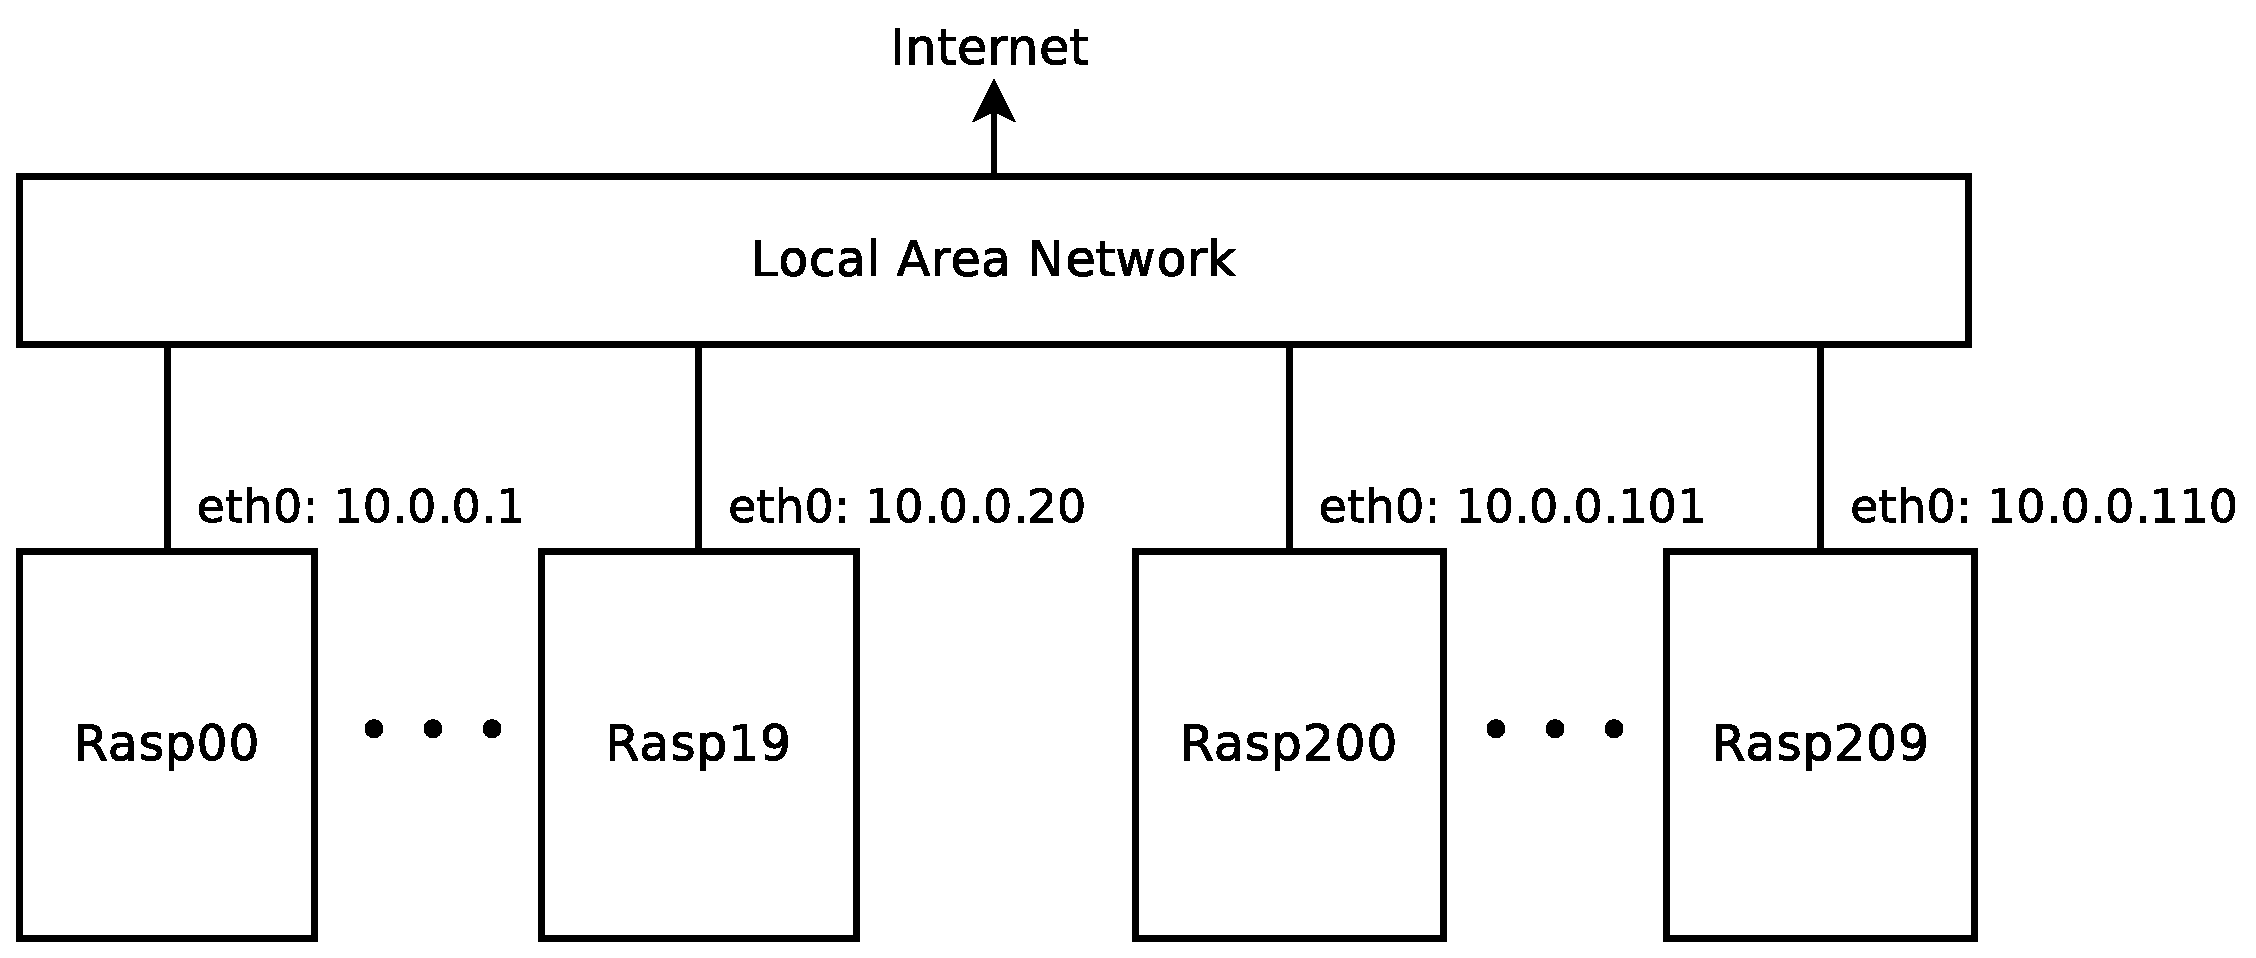
\includegraphics[width=0.6\textwidth]{images/testbed_setup.eps}
\caption{Testbed setup}
\label{fig:testbed_setup}
\end{figure}

This section will be used to present a Raspberry Pi testbed and the steps to
install and configure the individual devices.

The testbed is depicted in figure~\ref{fig:testbed_setup}. It consists of twenty
Raspberry Pi 1 model B rev 2 (Rasp\_01 to Rasp\_20) and 
ten Raspberry Pi 2 model b V1.1 (Rasp2\_01 to Rasp2\_10).

The goal is to configure all the devices identically with the same software
and configurations. There are however a few differences between them that we
need to take into account. E.g. hostname and network addresses.

The testbed will be used by students that might need to change how the
devices are work either temporary or permanently. We will illustrate how this
can be accomplished using an overlaying filesystem.

Finally, it should be possible to store data that are generated from
simulations on the memory cards that are in the individual Raspberry Pi.
%We using a overlaying filesystem that 
%We will illustrate
%how that can be done. In the case of temporary changes, it is important that
%all changes can be easily reverted. We put a \ac{RAM} filesystem on top of
%the the root filesystem to .
%the configure the
%devices to behave according to their test specifications. We
%will also present how that might be done.

%their linkings. That could be to change network config

%The goal is to configure all the devices to be as identical as possible. This
%means that it is desired to have the same software on every device, but  

The Raspberry Pis are all equipped with an ethernet interface (eth0) and
connected by wire to the university's \ac{LAN}. The university network
administration was provided
the \ac{MAC} addresses of the ethernet interfaces to automatically assign
the devices the desired \ac{IP} addresses as shown in the figure. In a personal
\ac{LAN}, another option could be to manually provide the devices with static
\ac{IP}s.
%that are
%assigned the \ac{IP} addresses in the figure and connected wired to the
%university's \ac{LAN}. 

We use standard usb power adapters to power the Raspberry Pis.

\subsubsection{Installing Raspbian}

To get started, we first need to install an \ac{OS} on the
Raspberry Pis. We will use Raspbian linux~\cite{raspbian}

We will use a desktop that has linux installed to download,
configure, and write the image to the memory cards.
%We have decided to use a linux desktop machine to create a
%common image of Raspbian Linux that can be used in any of the Raspberry Pis.

%for all devices. After the image has been configured it can be written to
%a memory card and used in any of the Raspberry Pis. This means that each
%device needs a memory card, but it does not matter which card is put into
%which device.

We have decided to go with Raspbian linux~\cite{raspbian} and
to install it on memory cards.


%There exists a number of ways to setup a testbed in a centralized manner.
%E.g. using e.g. \ac{NFS}.

There exists a number of ways to setup a testbed 

with multiple devices. We
have decided on a very simple approach of simply instal


- 
- Download image (wget)
- Update/Modify image (chroot)
- Burn image
- Bang! linux is running
- 

Open a terminal, and then...

hashmark (\#) means to perform operation as root, dollar (\$) means to perform operation as user

% Define variable]
\begin{lstlisting}[] 
$ export IMAGE="2016-05-27-raspbian-jessie-lite"
$ export WORKDIR="${HOME}/Raspbian"
\end{lstlisting}
\FloatBarrier



% Download and unpack image
\begin{lstlisting}[] 
$ mkdir -p ${WORKDIR}
$ cd ${WORKDIR}
$ wget http://downloads.raspberrypi.org/raspbian_lite/images/raspbian_lite-2016-05-31/${IMAGE}.zip
$ unzip ${IMAGE}.zip
\end{lstlisting}
\FloatBarrier


% Check out the image   % The dollar hack was to fix vim syntax
\begin{lstlisting}[literate={DOLLAR}{\$}1]
DOLLAR fdisk -lu ${IMAGE}.img
Disk 2016-05-27-raspbian-jessie-lite.img: 1.3 GiB, 1387266048 bytes, 2709504 sectors
Units: sectors of 1 * 512 = 512 bytes
Sector size (logical/physical): 512 bytes / 512 bytes
I/O size (minimum/optimal): 512 bytes / 512 bytes
Disklabel type: dos
Disk identifier: 0x6fcf21f3

Device                               Boot  Start     End Sectors  Size Id Type
2016-05-27-raspbian-jessie-lite.img1        8192  137215  129024   63M  c W95 FAT32 (LBA)
2016-05-27-raspbian-jessie-lite.img2      137216 2709503 2572288  1.2G 83 Linux
\end{lstlisting}
\FloatBarrier

We see that the boot and root partitions starts at sector 8192 and 137216 respectivly.
We also notice that each sector is 512 bytes.


On newer systems, we can mount the device easier using "losetup --show -f -P IMAGE"

Mount root partition:

\begin{lstlisting}[]
$ export ROOTDIR="${WORKDIR}/root"
$ mkdir -p ${ROOTDIR}
# mount -o loop,offset=$((137216*512)) ${IMAGE}.img ${ROOTDIR}
\end{lstlisting}
\FloatBarrier

Mount boot partition:
\begin{lstlisting}[]
# mount -o loop,offset=$((8192*512)) ${IMAGE}.img ${ROOTDIR}/boot
\end{lstlisting}
\FloatBarrier

We can now change all the files in the disk image.



\subsection{Configuring OS files and scripts}


% MAC and Hostname file
\Suppressnumber\begin{lstlisting}[]
<@\textcolor{gray}{\$\{ROOTDIR\}/home/pi/rasp\_config/nodes.csv}@>
<@\textcolor{gray}{
---------------------------------------------------------------}
\Reactivatenumber @>
# Ethernet MAC    Hostname
b8:27:eb:5b:da:20 rasp00
b8:27:eb:7b:c3:91 rasp01
b8:27:eb:54:9c:64 rasp02
b8:27:eb:95:bd:11 rasp03
\end{lstlisting}
\FloatBarrier


% Set hostname
\Suppressnumber\begin{lstlisting}[]
<@\textcolor{gray}{\$\{ROOTDIR\}/home/pi/rasp\_config/set\_hostname}@>
<@\textcolor{gray}{
---------------------------------------------------------------}
\Reactivatenumber @>
#!/usr/bin/env bash
mac=$(cat /sys/class/net/eth0/address)
hostname=$(grep $mac nodes.csv | cut -f2 -d' ')

# Assign hostname found in nodes.csv
if [ ! -z $hostname ]; then
    echo $hostname > /etc/hostname
    hostname $hostname
fi
\end{lstlisting}
\FloatBarrier



% Get the files
\begin{lstlisting}[]
$ wget http://kom.aau.dk/project/TuneSCode/rasp_config.zip
# unzip rasp_config.zip -d ${ROOTDIR}/home/pi/
\end{lstlisting}
\FloatBarrier


Call set\_hostname script at startup. We insert a line of code to call script in rc.local just after the initial comments (i.e. lines starting with \#).
\begin{lstlisting}[]
# line_number=$(egrep -n -m1 "(^[^#])|(^$)" ${ROOTDIR}/etc/rc.local | cut -d: -f1)
# sed -i "${line_number}c bash /home/pi/rasp_config/set_hostname" ${ROOTDIR}/etc/rc.local
\end{lstlisting}
\FloatBarrier
%$ line="bash /home/pi/.rasp_config/set_hostname"
%# awk -v text="$line" '!/^#/ && !p {print text; p=1} 1' ${ROOTDIR}/etc/rc.local > <@ \Suppressnumber @>
%    ${ROOTDIR}/etc/rc.local <@ \Reactivatenumber @>


All other files could be updated.

\subsection{Installation and Updating the image}

It may be desired to pre-install some programs in the image before it is
written to all the memory cards that goes into the Raspberry pis.
This can be done using QEMU Chroot (change root).
\url{https://wiki.archlinux.org/index.php/Raspberry_Pi}

\fxnote{Lets use RPi for Raspberry Pis throughout the paper!}
\fxnote{Which packages is required for this on debian/ubuntu?}


% CHROOT to OS image
\begin{lstlisting}[]
# apt-get install binfmt-support qemu qemu-user-static
# update-binfmts --importdir /var/lib/binfmts/ --import
# update-binfmts --display qemu-arm
# update-binfmts --enable qemu-arm
\end{lstlisting}
\FloatBarrier

% CHROOT to OS image
\begin{lstlisting}[]
# cd $ROOTDIR
# cp /etc/resolv.conf etc/resolv.conf
# cp /usr/bin/qemu-arm-static usr/bin
# mount -t proc proc proc/
# mount --rbind /sys sys/
# mount --rbind /dev dev/
# proot -q qemu-arm-static -S ${ROOTDIR}

ALTERNATIVE:
# chroot ${ROOTDIR} /usr/bin/qemu-arm-static /bin/bash
\end{lstlisting}
\FloatBarrier


% Optionally, we may create a unique prompt to indicate we have changed root
\begin{lstlisting}[]
# export PS1="(chroot) $PS1"
\end{lstlisting}
\FloatBarrier



% Update system
\begin{lstlisting}[]
# apt-get update
# apt-get upgrade
\end{lstlisting}
\FloatBarrier

Lets install some programs
% Install packages
\begin{lstlisting}[]
# apt-get install vim git
\end{lstlisting}
\FloatBarrier



\subsection{Installation an overlaying filesystem}

We use the code provided by 

Assumuing that we are still chrooted to the RPi image and the boot partition is mounted to /boot

% Get files
\begin{lstlisting}[]
# OVERLAYROOTDIR="/tmp/overlayroot"
# git clone https://github.com/chesty/overlayroot.git $OVERLAYROOTDIR
\end{lstlisting}
\FloatBarrier

% Install required packages
\begin{lstlisting}[]
# apt-get install busybox
\end{lstlisting}
\FloatBarrier

% Setup initramfs
\begin{lstlisting}[]
# cp ${OVERLAYROOTDIR}/hooks-overlay /etc/initramfs-tools/hooks/
# cp ${OVERLAYROOTDIR}/init-bottom-overlay /etc/initramfs-tools/scripts/init-bottom/
# echo "overlay" > /etc/initramfs-tools/modules
\end{lstlisting}
\FloatBarrier

% Tell uboot to load initramfs
\begin{lstlisting}[]
# echo "initramfs init.gz" > /boot/config.txt
\end{lstlisting}
\FloatBarrier

% Create an initramfs
\begin{lstlisting}[]
# mkinitramfs -o /boot/init.gz
# mkinitramfs -o /boot/init.gz -k 4.4.11+
\end{lstlisting}
\FloatBarrier

\subsection{Write image}

% Exit chroot, umount, and write to memory card
\begin{lstlisting}[]
# exit
# cd ..
# umount --recursive ${ROOTDIR}
# losetup -d WHICH_NUMBE.img of=/dev/mmcblk0 bs=4MR
# dd if=${IMAGE}.img of=/dev/mmcblk0 bs=4M
\end{lstlisting}
\FloatBarrier


\subsection{Kodo cross-compilation: From your PC to the Raspberry Pi}

Besides the previous description (\textbf{Include compiling Kodo from the
RasPi from the scratch}), the testbed administrator can compile Kodo in its
personal workstation and transfer the generated binaries directly to
a path in the Raspberry Pi. To achieve this, we get a toolchain that
contains the binaries for the \texttt{raspberry-gxx49-arm-g++} compiler
for the Raspberry Pi. Therefore, we strongly recommend any testbed
administrator to do the following procedure. In what follows, we provide
the instructions considering that the NFS server uses the \texttt{\$HOME}
directory as the working directory. However, the administrator may choose
some other working directory of its preference if desired.

\begin{enumerate}

\item Download the Raspberry Pi toolchain for 64-bit Linux from: \\
\texttt{http://buildbot.steinwurf.dk/toolchains/linux/} to your
\texttt{\$HOME} directory. \\

\item Extract the downloaded file locally in the NFS server. After
this operation, there should be a new directory for the toolchain
in the server. \\

\item Add the \texttt{bin} folder of the toolchain to the \texttt{PATH}
Linux environment variable of the server. This will help the server OS
to recognize the location of the compiler command, which will be needed
later. To do so, edit the \texttt{\$HOME/.profile} to add in a newline:
\texttt{PATH="\$PATH:\$HOME/raspberry-gxx49-arm/bin"}. Save the
\texttt{\$HOME/.profile}. \\

\item Restart the server session in order for the changes made in the
previous step take effect. To verify this, open a new terminal and type:
\texttt{raspberry-gxx49-arm-g++ --version}. A correct binary installation
should return an output similar to:

\texttt{raspberry-gxx49-arm-g++ (crosstool-NG 1.21.0) 4.9.3 20150311 (prerelease)
Copyright (C) 2014 Free Software Foundation, Inc.
This is free software; see the source for copying conditions.  There is NO
warranty; not even for MERCHANTABILITY or FITNESS FOR A PARTICULAR PURPOSE.} \\

\item Clone the Kodo repository in the server by executing: \\
\texttt{git clone git://github.com/steinwurf/kodo.git} in \texttt{\$HOME}. \textbf{Change the repo to kodo-rlnc or kodo-cpp since just raw kodo is going to be depreceated soon} \\

\item Navigate to the repository and configure \texttt{waf} by typing:
\texttt{python config.py} and select the 16th ``make specification'' file
for the Raspberry Pi, e.g. option \texttt{[16]cxx\_raspberry\_gxx49\_arm}
presented by the file.

This command configures \texttt{waf} to use the proper compiler and its
required flags to generate the binaries for the Raspberry Pi. If the
configuration was correct, the output will indicate:
\texttt{'configure' finished successfully (X.XXXs)}, where \texttt{X.XXX}
is total time in seconds for configuring the project in the server. \\

\item Execute \texttt{python waf build}. If the build process was
successful, the generated binaries for the Raspberry Pi should be located
in \texttt{build/cxx\_raspberry\_gxx49\_arm} in the Kodo repository.
\textbf{Indicate how the binary files should look like}.

Once this procedure is made, the testbed administrator can relocate the
generated binary files to Raspberry Pi's through the network as desired
by using the \texttt{scp} command during the configuration step.


\end{enumerate}

\subsection{Kodo Builds for the Raspberry Pi, Platform Support and Documentation}

You can check the build status of Kodo, Fifi and other relevant projects through
their respective repository master branch on our buildbot page
\cite{steinwurf2016buildbot}. Our buildbot displays the status of the builds for
Raspbian 8 and GCC 4.9 for the ARM architecture which is the relevant one for the
Raspberry Pi. At the link, you can check build status and build statistics. Also,
documentation about Kodo basics with a tutorial is available at \cite{kododocs}.
